% ============================================================================
\section{Supplementary Tables, Derivations, and Details}
% ============================================================================

\subsection{Notation and configuration}
\label{app:reference_tables}

\begin{table}[H]
\centering
\small
\caption{Notation and the values used in the four-teacher study.}
\label{tab:notation}
\begin{tabular}{cll}
\toprule
Symbol & Meaning & Value in this study \\
\midrule
$M$ & number of tasks and teachers & $4$ \\
$w_i$ & fixed objective weight & inverse initial loss, normalized \\
$G$ & micro-batches per optimizer step & $16$ \\
$b$ & prompts per micro-batch, one response each & $4$ \\
$m_i$ & task-$i$ micro-batch count & $2\leq m_i\leq8$ \\
$g_{i,s}$ & unweighted micro-batch gradient & from the backward pass \\
$D$ & AdamW diagonal scaling & $(\sqrt v+\epsilon)^{-1}$ \\
$e_i,\ \widehat e_i$ & scaled one-micro-batch noise; its within-step estimate & estimated each step \\
$\tau_i,\ C$ & time per task-$i$ micro-batch; fixed time per step & exponential averages \\
$H$ & predicted variance ratio relative to Uniform & $H\leq2$ \\
\bottomrule
\end{tabular}
\end{table}

\begin{table}[H]
\centering
\footnotesize
\caption{Four-teacher MOPD configuration.}
\label{tab:pipeline}
\begin{tabular}{p{0.20\linewidth}p{0.72\linewidth}}
\toprule
Component & Configuration \\
\midrule
Student & Qwen3-1.7B \citep{qwen2025qwen3};
\missing{exact checkpoint revision; Base/SFT/Instruct status; initial scores} \\
Teachers & One fixed specialist for each of math, code, instruction following,
and science; \missing{teacher names, sizes, revisions, origins, and same-origin
status} \\
Training prompts & $16{,}000$ unique prompts per task, shuffled once and read
without replacement; \missing{dataset names, versions, licenses, and filters} \\
Rollout and loss & One response per prompt; one update per rollout batch;
sampled-token reverse KL, averaged over valid tokens and then prompts;
maximum response length $8{,}192$, truncated responses kept;
\missing{temperature, ratio-truncation rule, and observed truncation rate by
task} \\
Step and budget & $b=4$ prompts per micro-batch, $G=16$ micro-batches per
step, $500$ steps, and $32{,}000$ attempted responses; $2\leq m_i\leq8$ \\
Optimization & AdamW; inverse-initial-loss objective weights fixed before
training; \missing{learning rate and schedule, $\beta_1$, $\beta_2$,
$\epsilon$, weight decay, gradient clipping, precision, and sharding} \\
Evaluation & Held-out teacher loss on $128$ fixed prompts per task from
checkpoints every $50$ steps; MATH-500, LiveCodeBench slice, IFBench,
GPQA-Diamond; \missing{benchmark versions and decoding settings} \\
Seeds & $3$ for Uniform and GPAS; $1$ for Cost-GPAS and RawNoise \\
System & At most one teacher loaded at a time, in a fixed cyclic order;
\missing{GPU type and count, inference engine, software revisions, and GPU
hours per run} \\
\bottomrule
\end{tabular}
\end{table}

\subsection{One-step variance criterion}
\label{app:descent}

Let $D$ be fixed within the step. If $F$ is $L$-smooth and
$\theta'=\theta-\eta DA$, then
\begin{equation}
    \mathbb E[F(\theta')]
    \leq F(\theta)-\eta\nabla F^\top D\nabla F
    +\frac{\eta^2L}{2}
      \left(\|D\nabla F\|_2^2+V(m)\right).
    \label{eq:one_step_descent}
\end{equation}
For a fixed student state, $D$, and step size, only $V(m)$ depends on the
allocation. This local bound motivates the variance criterion; the
end-to-end experiment includes momentum and gradient clipping.

\subsection{Gradient variance, its estimate, and the allocation rules}
\label{app:allocation_proofs}

Independence across tasks and micro-batches gives
\begin{equation}
\mathbb E\|D(A-\mathbb E[A])\|_2^2
=\sum_iw_i^2\,\mathbb E\|D(\bar g_i-\mathbb E[g_i])\|_2^2
=\sum_i\frac{w_i^2}{m_i}\,\mathbb E\|D(g_i-\mathbb E[g_i])\|_2^2,
\end{equation}
which is Equation~\ref{eq:batch_variance}. Within a step,
$\sum_s\|D(g_{i,s}-\bar g_i)\|_2^2=\sum_s\|Dg_{i,s}\|_2^2-m_i\|D\bar g_i\|_2^2$,
so Equation~\ref{eq:noise_estimate} is the usual unbiased sample variance
summed over the scaled coordinates and is defined whenever $m_i\geq2$.

Write $q_i=w_i\sqrt{e_i}$. With equal micro-batch cost, the Cauchy--Schwarz
inequality
\begin{equation}
\Bigl(\sum_i m_i\Bigr)\Bigl(\sum_i\frac{q_i^2}{m_i}\Bigr)
\geq\Bigl(\sum_i q_i\Bigr)^2
\end{equation}
holds with equality at $m_i\propto q_i$, which is GPAS. With task-dependent
cost and zero fixed overhead,
\begin{equation}
\Bigl(\sum_i m_i\tau_i\Bigr)\Bigl(\sum_i\frac{q_i^2}{m_i}\Bigr)
\geq\Bigl(\sum_i q_i\sqrt{\tau_i}\Bigr)^2,
\end{equation}
with equality at $m_i\propto q_i/\sqrt{\tau_i}$. For $C>0$, Cost-GPAS
evaluates Equation~\ref{eq:batch_cost_objective} over the feasible integer
counts. In both rules the continuous counts are clipped to
$[m_{\min},m_{\max}]$ by solving for the scale at which the clipped counts sum
to $G$, and the result is rounded by largest remainder.

\subsection{Allocation and AdamW's second moment}
\label{app:moment_target_proof}

For a fixed allocation, assume task-$i$ micro-batch gradients are independent
with mean $h_i$ and coordinatewise variance $\sigma_i^2$. Equation
\ref{eq:batch_gradient_observation} gives
\begin{equation}
    \mathbb E[A]=\sum_iw_i h_i,
    \qquad
    \mathbb E[A^2]=\Bigl(\sum_iw_i h_i\Bigr)^2
    +\sum_i\frac{w_i^2}{m_i}\sigma_i^2,
    \label{eq:conventional_batch_second_moment}
\end{equation}
so the noise term of AdamW's second-moment observation depends on the
allocation, as it does under any change of batch composition. Within the
count bounds each task's term lies between $0.5\times$ and $2\times$ its
Uniform value, and the observation enters the update through the square root
of an exponential average, so the update magnitude in a noise-dominated
coordinate changes by less than a factor of $\sqrt2$ in the worst case. The
experiments use conventional AdamW.

An allocation-independent observation is available if desired:
\begin{equation}
    U=\sum_{i=1}^M\frac{w_i}{m_i}\sum_{s=1}^{m_i}g_{i,s}^2,
    \qquad
    \mathbb E[U/G]=\frac1G\sum_iw_i\bigl(h_i^2+\sigma_i^2\bigr),
    \label{eq:taskwise_square_observation}
\end{equation}
whose expectation does not depend on $m$. At proportional allocation
$m_i=Gw_i$ its noise term equals that of
Equation~\ref{eq:conventional_batch_second_moment}; using $U$ without the
$1/G$ factor would enlarge the target by about $G$ and shrink updates by about
$\sqrt G$ in noise-dominated coordinates. In the controlled check below,
reallocating from Uniform to GPAS changes the conventional $A^2$ observation
by $0.543$ in relative norm (calculated $0.542$) and the $U/G$ observation by
$0.0009$ (calculated $0$).

\subsection{Controlled calculation}
\label{app:controlled}

The controlled check uses three Gaussian micro-batch gradients in three
coordinates and a diagonal AdamW scaling that reverses their noise ranking.
Every step contains $G=16$ micro-batches with $2\leq m_i\leq12$. Bounded
rounding gives counts $(6,5,5)$ for Uniform, $(11,3,2)$ for RawNoise,
$(3,3,10)$ for GPAS, and $(3,5,8)$ for zero-overhead Cost-GPAS. All methods
use the same fixed weights and common random numbers over $20{,}000$ trials.
GPAS attains $0.679\times$ Uniform's scaled variance (calculated $0.681$),
RawNoise $2.316\times$, and Cost-GPAS a time--variance product of
$0.857\times$ Uniform (calculated $0.854$). The second-moment panel uses
$200{,}000$ simulated steps.

\begin{figure}[H]
    \centering
    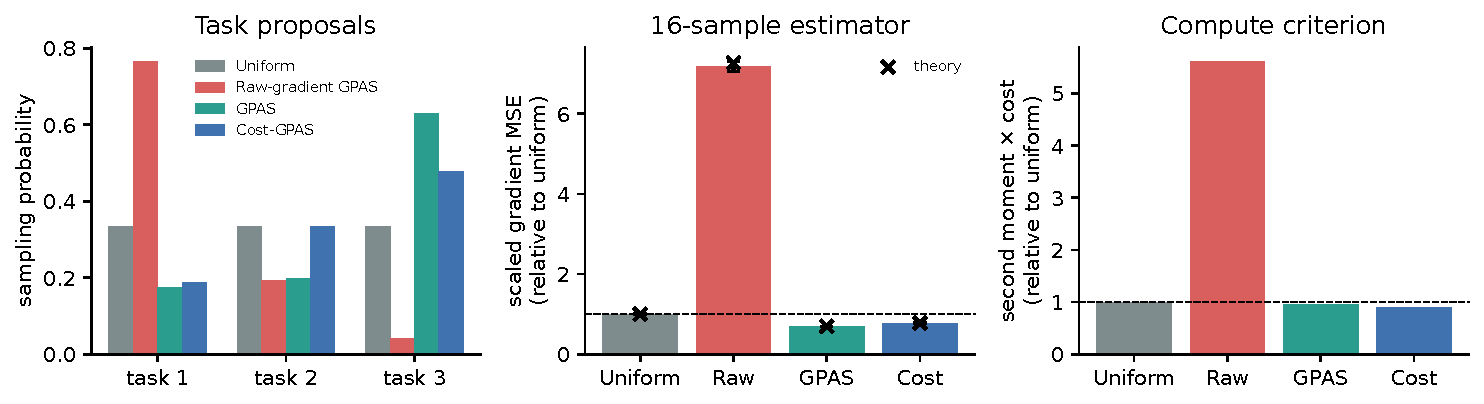
\includegraphics[width=0.98\linewidth]{figures/controlled_optimizer_sampling.pdf}
    \caption{Controlled checks. Bars are Monte Carlo estimates and crosses are
    calculated values. GPAS uses AdamW-scaled within-task noise; Cost-GPAS also
    uses task cost. The last panel compares second-moment observations after
    an integer reallocation.}
    \label{fig:controlled_checks}
\end{figure}

\subsection{MOPD loss and micro-batch normalization}
\label{app:opd_estimators}

For a student-generated prefix $z$, write
$q_v=\pi_\theta(v\mid z)$ and $t_v=T_i(v\mid z)$. The sampled-token reverse-KL
score is
\begin{equation}
    \operatorname{sg}\!\left[\log\frac{q_V}{t_V}\right]
    \nabla_\theta\log q_V,\qquad V\sim q.
\end{equation}
The implementation averages valid tokens within one response and then the
$b=4$ responses from distinct prompts in a micro-batch. Any configured
importance-ratio truncation is applied before these means; the fixed-objective
factor $w_i/m_i$ is applied after them. There is no groupwise advantage
normalization and no outcome-reward term.

\subsection{Held-out gradient variance protocol}
\label{app:heldout}

At each of three Uniform checkpoints (steps \missing{50, 250, 500}) and for
each task, we generate $32$ fresh micro-batches from the held-out prompts and
record $\|Dg_{i,s}\|_2^2$ and $\|D\bar g_i\|_2^2$ for each half, with $D$ from
the checkpoint's AdamW state. Half $\mathcal A$ gives
$\widehat e^{\mathcal A}_i$, from which each rule computes its allocation
$m^{\mathcal A}$; half $\mathcal B$ gives $\widehat e^{\mathcal B}_i$, and the
held-out variance of that allocation is
$\sum_iw_i^2\widehat e^{\mathcal B}_i/m^{\mathcal A}_i$, reported relative to
the same quantity at Uniform counts. We exchange the halves and average. The
estimator error $|\widehat e^{\mathcal A}_i-\widehat e^{\mathcal B}_i|
/\widehat e^{\mathcal B}_i$ is also computed from subsets of two and four
micro-batches to match the online estimate. Only scalar norms are stored.

\subsection{System timing and logs}
\label{app:system_details}

For each task in a step, the log records teacher load and offload time,
rollout, scoring, backward, and optimizer time, peak memory, attempted
responses, and valid and generated tokens. $\tau_i$ is the rollout, scoring,
and backward time of task $i$'s micro-batches divided by $m_i$; $C$ is the
remaining step time, including teacher loading and the optimizer update.
GPU hours include all loading and waiting time. Checkpoints store the
allocation, noise estimates, timing averages, and prompt positions, and a
resume test reproduces the next allocation and parameter update. Under
concurrent teacher serving the step time is closer to $C+\max_i m_i\tau_i$
than to the serial sum; the fixed-objective scaling and GPAS are unchanged,
and Cost-GPAS should use the step-time model fitted for that layout.

\subsection{Full task-level trajectories}

\begin{figure}[H]
    \centering
    \missingfigure[0.18\textheight]{Insert per-task held-out and training
    losses, prompt consumption, response length and truncation, count-bound
    occupancy, and step-time quantiles from the released logs.}
    \caption{Task-level training and system traces.
    \missing{Replace after the four-teacher runs finish.}}
    \label{fig:appendix_task_curves}
\end{figure}
